\section{Experiments}
\label{sec:experiments}


\subsection{Experimental Settings} \label{sec:experimental_settings}
\noindent \textbf{Benchmarks.}
To demonstrate the effectiveness and efficiency of our proposed AOT, we evaluate our method on four commonly used video understanding benchmarks: MVBench~\cite{li2024mvbench}, EgoSchema~\cite{mangalam2023egoschema}, LongVideoBench~\cite{wu2024longvideobench}, and VideoMME~\cite{fu2025video}. Comprising videos of various lengths and complex scenarios, these benchmarks provide a comprehensive testbed for demonstrating the effectiveness and generalization of our method.



\begin{table*}[t]
\centering
% \vspace{-0.8cm}
\caption{ 
Comparison of state-of-the-art methods on LLaVA-OneVision~\cite{li2024llava} across video benchmarks. The best performance among those with similar retention ratios is highlighted in \textbf{bold}, while the second best will be denoted as \underline{underlined}.
}
\vspace{-0.2cm}
\resizebox{\textwidth}{!}{%
\begin{tabular}{l|ccc|cccc|cc}
\toprule
\multirow{2}{*}{Method} &
\multirow{2}{*}{\makecell{Prefilling\\FLOPs (T) $\downarrow$}} & \multirow{2}{*}{\makecell{FLOPs\\Ratio $\downarrow$}} & \multirow{2}{*}{\makecell{Before LLM\\Retained Ratio}}
& \multirow{2}{*}{\makecell{MVBench\\ $\uparrow$}} & \multirow{2}{*}{\makecell{EgoSchema\\ $\uparrow$}} & \multirow{2}{*}{\makecell{LongVideo\\Bench $\uparrow$}} & \multirow{2}{*}{\makecell{VideoMME\\ $\uparrow$}} & \multicolumn{2}{c}{Avg. $\uparrow$}  \\
&&&&&&&& Score & \% \\
\midrule
\rowcolor{gray!20} 
LLaVA-OV-7B & 40.8 & 100\% & 100\% 
& 58.3 & 60.4 & 56.4 & 58.6 & 58.4 & 100 \\ %
FastV~\cite{chen2024image} & 9.3 & 22.8\% & 100\%
& 55.9 & 57.5 & \textbf{56.7} & 56.1 & 56.5 & 96.7 \\ %
PDrop~\cite{xing2024pyramiddrop} & 10.5 & 25.7\% & 100\%
& 56.1 & 58.0 & 54.1 & 56.4 & 56.2 & 96.2 \\
DyCoke \cite{tao2025dycoke} & 8.7 & 21.3\% & 25\% & 53.1 & 59.5 & 49.5 & 54.3 & 54.1 & 92.6 \\

VisionZip~\cite{yang2025visionzip} & 8.7 & 21.3\% & 25\%
& \underline{57.9} & \underline{60.3} & \underline{56.5} & \textbf{58.2} & \underline{58.2} & \underline{99.7} \\ %

PruneVid~\cite{huang2024prunevid} & 8.7 & 21.3\% & 25\%
& 57.4 & 59.9 & 55.7 & 57.4 & 57.6 & 98.6 \\ %

FastVID~\cite{shen2025fastvid} & 8.7 & 21.3\% & 25\%
& 56.5 & - & 56.3 & \underline{58.0} & - & - \\

\textbf{AOT} & 8.7 & 21.3\% & 25\%
& \textbf{58.7} & \textbf{61.3} & 56.3 & 57.5 & \textbf{58.5} &  \textbf{100.0} \\ %
\midrule
VisionZip~\cite{yang2025visionzip} & 7.0 & 17.2\% & 20\%
& \underline{57.7} & \underline{59.8} & 55.2 & \textbf{57.9} & \underline{57.7} & \underline{98.8} \\ %

PruneVid~\cite{huang2024prunevid} & 7.0 & 17.2\% & 20\%
& 57.2 & 59.7 & 54.7 & 56.9 & 57.1 & 97.8 \\ %

FastVID~\cite{shen2025fastvid} & 7.0 & 17.2\% & 20\%
& 56.3 & - & \textbf{57.1} & \textbf{57.9} & - & - \\

\textbf{AOT} & 7.0 & 17.2\% & 20\%
& \textbf{58.1}  & \textbf{61.3} & \underline{56.2} & \underline{57.2} & \textbf{58.2} & \textbf{99.7} \\ %
\midrule
VisionZip~\cite{yang2025visionzip} & 5.2 & 12.7\% & 15\%
& 56.5 & \underline{59.8} & 54.4 & 56.1 & 56.7 & 97.1 \\ %

PruneVid~\cite{huang2024prunevid} & 5.2 & 12.7\% & 15\%
& \underline{56.8} & 59.7 & \underline{55.4} & \underline{56.6} & \underline{57.1} & \underline{97.8} \\ %

FastVID~\cite{shen2025fastvid} & 5.2 & 12.7\% & 15\% & 56.0 & - & \textbf{56.2} & \textbf{57.7} & - & - \\

\textbf{AOT} & 3.4 & 8.3\% & 15\%
& \textbf{57.8}  & \textbf{61.3} & 55.2 & \underline{56.6} & \textbf{57.7} & \textbf{98.8} \\ %
\midrule
VisionZip~\cite{yang2025visionzip} & 3.4 & 8.3\% & 10\% 
& 53.5 & 58.0 & 49.3 & 53.4 & 53.5 & 91.6 \\ %

PruneVid~\cite{huang2024prunevid} & 3.4 & 8.3\% & 10\% 
 & \underline{56.2} & \underline{59.8} & \underline{54.5} & 56.0 & \underline{56.6} & \underline{96.9} \\ %

FastVID~\cite{shen2025fastvid} & 3.4 & 8.3\% & 10\% 
& 55.9 & - & \textbf{56.3} & \textbf{57.3} & - & - \\

\textbf{AOT} & 5.2 & 12.7\% & 10\%
& \textbf{57.0}  & \textbf{60.6} & 54.2 & \underline{56.1} & \textbf{57.0} & \textbf{97.6} \\ %
% \midrule
\bottomrule

\end{tabular}
}
\label{tab:ov_benchmark}
% \vspace{-4mm}
\vspace{-0.2cm}
\end{table*}



\begin{table*}[t]
% \vspace{-2mm}
\centering
\caption{Comparison of state-of-the-art methods on LLaVA-Video~\cite{zhang2024video} across video benchmarks. The best performance among those is highlighted in \textbf{bold}, while the second best will be denoted as \underline{underlined}, demonstrating consistent effectiveness.
}
\vspace{-0.2cm}
\resizebox{\textwidth}{!}{%
\begin{tabular}{l|ccc|cccc|cc}
\toprule
\multirow{2}{*}{Method} &
\multirow{2}{*}{\makecell{Prefilling\\FLOPs (T) $\downarrow$}} & \multirow{2}{*}{\makecell{FLOPs\\Ratio $\downarrow$}} & \multirow{2}{*}{\makecell{Before LLM\\Retained Ratio}}
& \multirow{2}{*}{\makecell{MVBench\\ $\uparrow$}} & \multirow{2}{*}{\makecell{EgoSchema\\ $\uparrow$}} & \multirow{2}{*}{\makecell{LongVideo\\Bench $\uparrow$}} & \multirow{2}{*}{\makecell{VideoMME\\ $\uparrow$}} & \multicolumn{2}{c}{Avg. $\uparrow$}  \\
&&&&&&&& Score & \% \\
\midrule
 \cellcolor{gray!20}{LLaVA-Video-7B} & \cellcolor{gray!20}{80.2} & \cellcolor{gray!20}{100\%} & \cellcolor{gray!20}{100\%} 
 & \cellcolor{gray!20}{60.4} & \cellcolor{gray!20}{57.2} & \cellcolor{gray!20}{58.9} & \cellcolor{gray!20}{64.3} & \cellcolor{gray!20}{60.2} & \cellcolor{gray!20}{100} \\ %

 FastV~\cite{chen2024image} & 17.1 & 21.3\% & 100\% 
& 54.3 & 54.1 & \underline{55.0} & 58.8 & 55.6 & 92.4 \\ %

 PDrop~\cite{xing2024pyramiddrop} & 19.5 & 24.3\% & 100\% 
& 55.9 & 54.3 & 54.7 & \underline{61.9} & \underline{56.7} & \underline{94.2} \\ %

 VisionZip~\cite{yang2025visionzip} & 9.3 & 18.9\% & 25\%
& \underline{56.7} & \underline{54.7} & 54.7 & 60.7 & \underline{56.7} & \underline{94.2} \\ %

 DyCoke~\cite{yang2025visionzip} & 9.3 & 18.9\% & 25\%
& 50.8 & - & 53.0 & 56.9 & - & - \\ %

 \textbf{AOT} & 9.3 & 18.9\% & 25\%
& \textbf{58.8}  & \textbf{55.4} & \textbf{56.2} & \textbf{62.4} & \textbf{58.2} & \textbf{96.7} \\ %

\hline

 VisionZip~\cite{yang2025visionzip} & 9.3 & 11.6\% & 15\%
& \underline{56.7} & \underline{54.7} & \underline{54.7} & \underline{60.7} & \underline{56.7} & \underline{94.2} \\ %

 \textbf{AOT} & 9.3 & 11.6\% & 15\%
& \textbf{57.8}  & \textbf{55.2} & \textbf{55.0} & \textbf{62.0} & \textbf{57.5} & \textbf{95.5} \\ %
\bottomrule



\end{tabular}
}%
\label{tab:diff_backbone}
% \vspace{-2mm}
\vspace{-0.4cm}
\end{table*}



\noindent \textbf{Implementation Details.}
\label{sec:implementation_details}
Our method is implemented on LLaVA-OneVision-7B~\cite{li2024llava} and LLaVA-Video-7B~\cite{zhang2024video} models. Both evaluation and inference use NVIDIA A100 GPUs. Inference cost is measured by prefilling FLOPs, with baselines configured for comparable FLOPs (see in the appendix). The number of intra-frame token anchors is set to be 126 for a 10\% token retention budget. Both intra- and inter-frame Sinkhorn-Knopp iterations are conducted with 100. The weighting coefficient $\lambda_{intra}$ and $\lambda_{inter}$ are set to default 1.0, otherwise stated.
Following official practice, LLaVA-OneVision models utilize 32 input video frames ($N_v$ = 196), while LLaVA-Video uses 64 sampled frames ($N_v$ = 169). All benchmarks are conducted using LMMs Eval~\cite{zhang2025lmms,li2024lmms} to report the results.



\noindent \textbf{Compared Baselines.}
We evaluate our proposed \textbf{\textit{AOT}} against six representative training-free approaches.
(1) FastV~\cite{chen2024image}, which selects salient visual tokens during prefilling based on attention guidance between predicted tokens and vision tokens;
(2) PDrop~\cite{xing2024pyramiddrop}, which discards visual tokens across hierarchical LLM blocks under the guidance of image and instruction tokens;
(3) VisionZip~\cite{yang2025visionzip}, which performs spatial token merging before feeding visual tokens into the LLM;
(4) DyCoke~\cite{tao2025dycoke}, which integrates temporal token merging before LLM with adaptive KV cache pruning during decoding;
(5) PruneVid~\cite{huang2024prunevid}, which reduces redundancy via jointly spatial and temporal token clustering;
and (6) FastVID~\cite{shen2025fastvid}, a recent method that segments videos into clips and applies density-aware token pruning.



\noindent \textbf{Inference Cost Analysis.}
\label{sec:inference_cost}
In this section, we investigate the FLOPs of the LLM backbone by counting the cost of each Transformer layer (MHA+FFN). Following~\cite{chen2024image,xing2024pyramiddrop,tao2025dycoke,shao2025holitom}, processing $n_i$ vision tokens at layer $i$ with hidden size $d$ and FFN width $m$ costs $4n_i d^2 + 2n_i^2 d + 2n_i d m$ FLOPs.
For an LLM with $T$ layers, the prefilling and decoding FLOPs can be computed as:
\begin{align}
    F_{\text{pre}}
    &= \sum_{i=1}^T \big(4n_i d^2 + 2n_i^2 d + 2n_i d m\big),\\
    F_{\text{dec}}
    &= \sum_{i=1}^T
    R\Big((4d^2 + 2d m) + 2\big(d n_i + \tfrac{1}{2}d(R+1)\big)\Big),
\end{align}
and the total cost is $F_{\text{pre}} + F_{\text{dec}}$.
With token generation number $R=100$, the decoding term contributes only about \textbf{2\%} of the total FLOPs in video LLMs, showing that computation is dominated by the prefilling stage. Therefore, reducing visual tokens \textit{before} feeding them into the LLM strikes significantly larger savings than pruning applied only inside the early layers of the LLM.



\subsection{Main Results}
\label{sec:main_results}

\noindent \textbf{Results on LLaVA-OneVision.} 
As shown in the Table.~\ref{tab:ov_benchmark}, we conduct AOT evaluations on various video benchmarks against state-of-the-art approaches on the LLaVA-OneVision 7B model, comparing the performances and analyzing the inference cost (so-called FLOPs) under various token retention budgets (25\%, 20\%, 15\%, and 10\%) before feeding the visual tokens into LLM for subsequent processing. Inner-LLM pruning methods, such as FastV~\cite{chen2024image} and PDrop~\cite{xing2024pyramiddrop}, often struggle to balance performance and efficiency, especially at lower token retention ratios (25\%). DyCoke~\cite{tao2025dycoke}, which segments video frames into groups of 4 and prunes all but the first frame, is limited by its design, capping its lowest retention ratio at 25\%. Spatial pruning methods like VisionZip~\cite{yang2025visionzip} show a significant performance drop (up to 8.4\%) at 10\% retention. This decline can be attributed to relying solely on spatial compression, which is less effective at preserving crucial spatiotemporal information needed for performance under aggressive pruning. Notably, even after
pruning \textbf{90.0\%} of the visual tokens, our AOT preserves averaged \textbf{97.6\%} of the vanilla model’s performance.
This demonstrates the superior robustness and adaptability of our approach compared to existing methods.



\noindent \textbf{Results on LLaVA-Video.} Table.~\ref{tab:diff_backbone} presents our AOT's performance on LLaVA-Video 7B model. 
%
LLaVA-Video-7B poses a greater compression challenge due to its higher initial pooling rate (169~\textit{vs.}~196 tokens for each frame in LLaVA-OneVision). Despite this, our method achieves a reduction to just 15\% of the original FLOPs, retaining 95.5\% performance and outperforming existing methods. 
Generally speaking, obtaining significant token compression with minimal performance decrease is indeed more difficult for LLaVA-Video 7B than for LLaVA-OneVision 7B.


\noindent \textbf{Scaling Input with more frames.}
To validate the performance fluctuation when varying input frames, we conduct experiments with increasing input frames to present the robust improvements of our method in Fig.~\ref{fig:scaling_frames}. A crucial challenge for video LLMs is that uniformly and sparsely sampled frames may lose essential visual information to obtain accurate answers. 
%
Fig.~\ref{fig:scaling_frames} illustrates that our approach consistently surpasses other compression methods across frame rates. 
At the sparse 16 sampled frames that contain less temporal redundancy, our AOT still transcends all other compression approaches. With denser 64 frames, thanks to our intra- and inter-level optimal token pruning, our method showcases more efficient and effective performances over the vanilla model. Moreover, when inputting with 128 frames, our token reduction method maintains an approximate context length, whereas the vanilla models suffer from maximum context length limitations. This further demonstrates the superiority of our proposed AOT that excels at tasks requiring extensive spatiotemporal context or answering complex questions with long text.



\noindent \textbf{Superior Performances after Token Reduction.}
As shown in Table.~\ref{tab:ov_benchmark} and Fig.~\ref{fig:scaling_frames}, we can find that models utilizing our token reduction can surpass the vanilla models on some benchmarks. This elucidates that there is excessive, irrelevant, or redundant information acting as noise, inducing useless visual cues for effective and efficient abstraction. The massive visual information misguides the subsequent LLM to focus on the critical parts, hence resulting in degraded results. Rather than directly removing unimportant or merging highly similar tokens, our method exploits optimal transport to comprehensively mine out informative signals from these tokens that consist of essential semantic and context to boost the selected token anchors, via a transport-weighted aggregation. In this way, the results highlight the efficacy of our method in aggregating or \textit{distilling} key visual information and further globally optimal refinement for better LLM processing, while we present qualitative visualizations in Fig.~\ref{fig:vis_cases}.



\subsection{Efficiency Analysis Sinkhorn-Knopp Iteration.} 
As shown in Table.~\ref{tab:ota_time}, we measure time consumption under 32 frames scenario using LLaVA-OneVision 7B on one single A100 GPU in terms of optimal transport using Sinkhorn-Knopp Iteration. We can see that with 100 iterations, the computational time for Intra-Frame OT takes around 0.51 milliseconds while 1.60 milliseconds to finish Inter-Frame OT, summing up to nearly 2.11 milliseconds which takes less than \textbf{1\%} of total inference time. For VisionZip~\cite{yang2025visionzip}, PruneVid~\cite{huang2024prunevid}, and our proposed AOT require token pre-processing before LLM, which introduces extra time. However, our method constructs a sparse and fixed number of tokens per frame as token anchors, while PruneVid produces a variable number of tokens per frame that complicates the batch processing acceleration, inevitably inducing extra computation overhead.


\subsection{Ablation Studies}
\label{sec:ablatives}

In this section, we conduct ablation studies on LLaVA-OneVision 7B by setting the token retention budget at 10\% to gradually demonstrate the improvements from each of our proposed components.


\noindent \textbf{Ablation on Intra-Frame Token Anchors Selection.}
To validate the effectiveness of the Local-Global token anchors establishment, shown in Table.~\ref{tab:ablations}, despite leveraging global-level anchors only can reach competitive performances across video benchmarks after employing our AOT, combining both global and local anchors achieves the best, demonstrating the effectiveness of retaining semantically important and spatially diverse token candidates.

\begin{figure}[t]
    % \vspace{0.5cm}
    \centering
    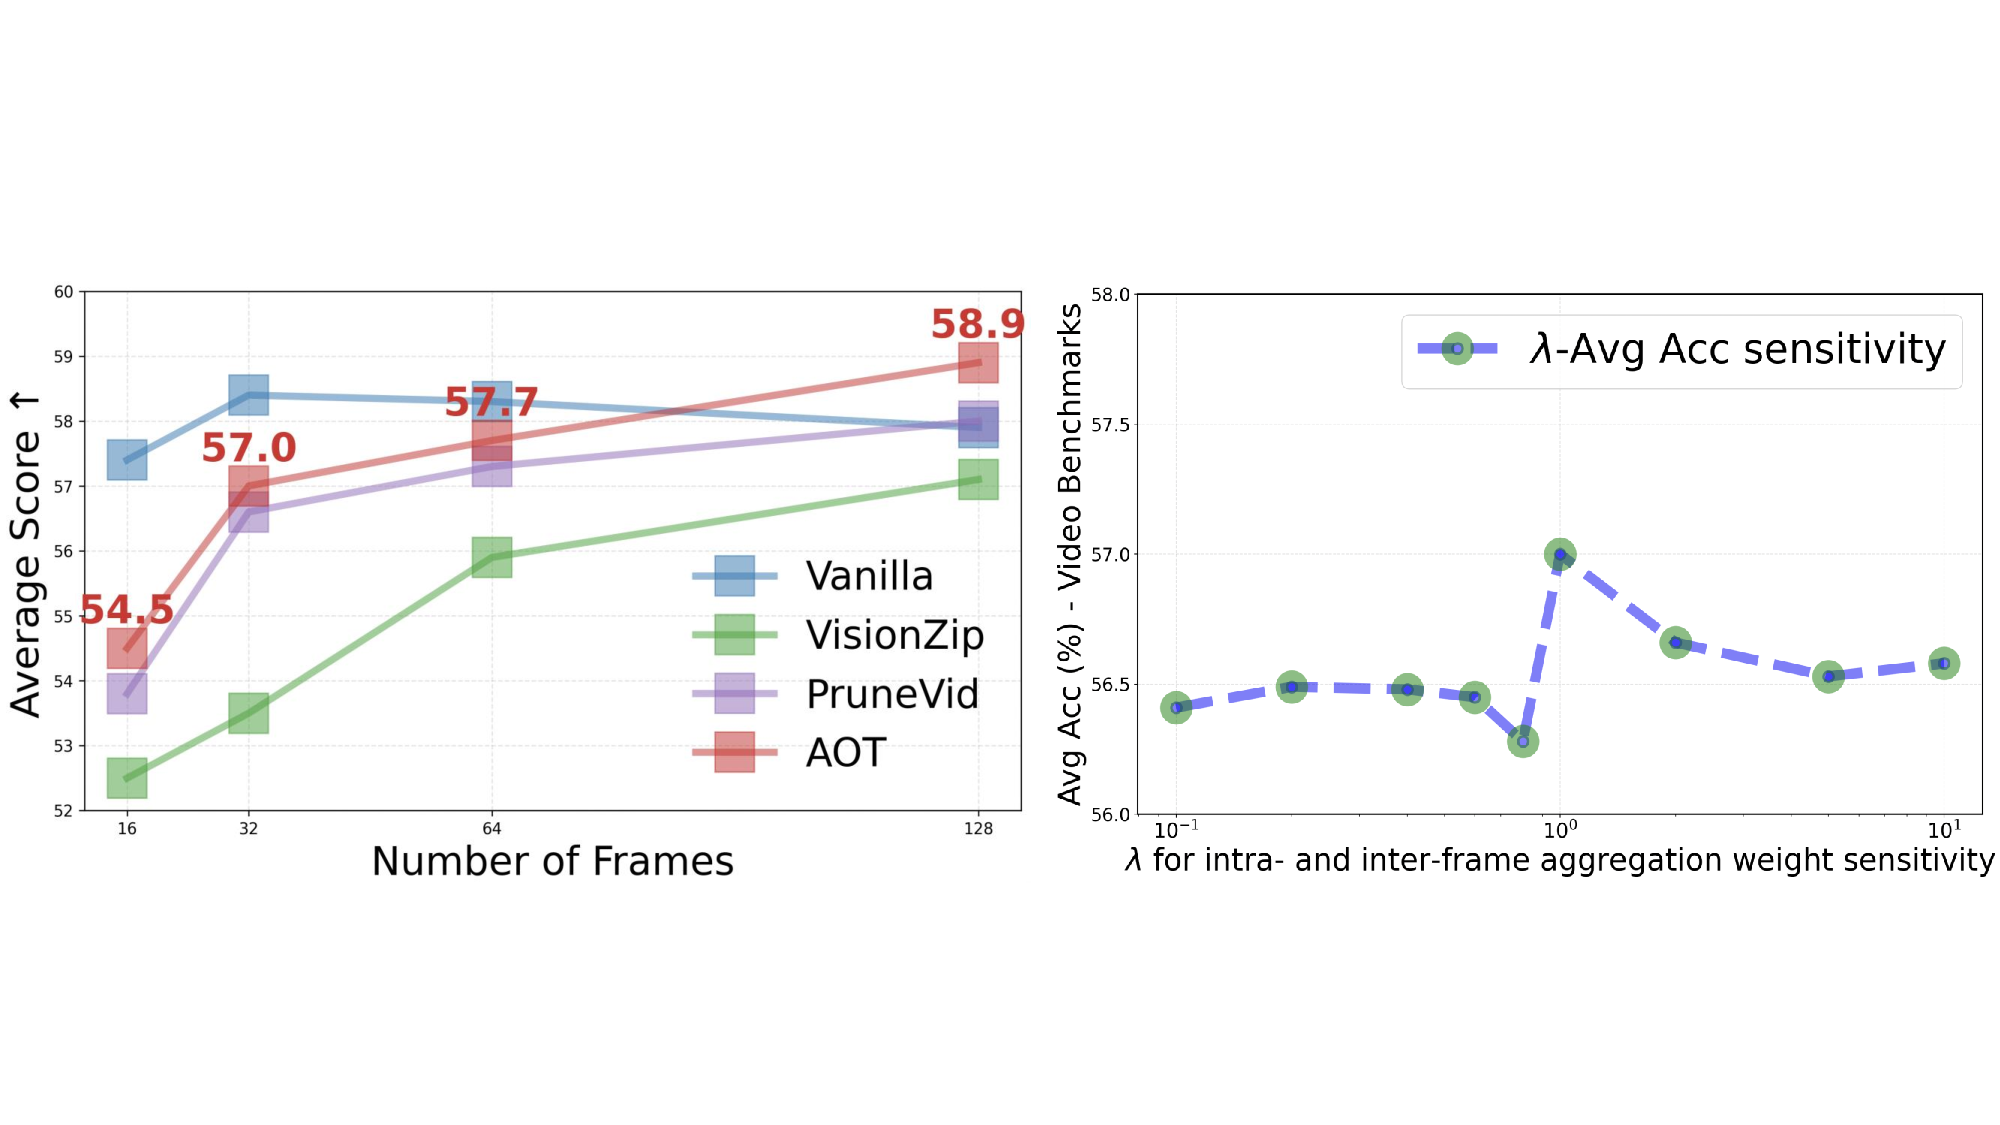
\includegraphics[width=1.0\linewidth]{figs/cvpr2026_frames.pdf}
    % \vspace{-0.6cm}
    \vspace{-0.5cm}
    \caption{\textbf{Left:} scaling with more frames leads to more efficient and effective visual information abstraction. \textbf{Right:} sensitivity analysis of weighting coefficient controlling contextual contribution with consistent configuration, $\lambda_{intra}$ and $\lambda_{inter}$.}
    \label{fig:scaling_frames}
    \vspace{-0.4cm}
\end{figure}



\noindent \textbf{Ablation on OT for Token Reduction.} In Table.~\ref{tab:ablations}, we can also observe that without optimal transport to aggregate comprehensive semantics and context from pruned tokens, the model will result in degraded performances, particularly for aggressive token compression, elucidating the importance of these subtle yet informative context.



\noindent \textbf{Ablation on OT for Intra-Frame and Inter-Frame.}
We conduct experiments in Table.~\ref{tab:ablations} that integrating the optimal transport from both intra- and inter-frame optimization helps aggregate necessary semantics and contexts from merging or removing tokens into selected token anchors to process complex videos better, instead of applying simple merging or removing them. This further demonstrates our approach significantly accelerates Video LLM inference while preserving both temporal and visual integrity.



\noindent \textbf{Ablation on Aggregation for Token Anchors.}
In Table.~\ref{tab:merging_strategy}, we further conduct studies to validate the effectiveness of aggregating the information from unimportant and very similar tokens through the optimized transport plan $T$, including intra- and inter-frame. Compared with no merging and cosine similarity weighting, the transported-weighting $T$ showcases superior token compression performances, which demonstrates the efficacy of local-global Optimal Transport aggregation in this paper.


\noindent \textbf{Sensitivity on Weightings $\lambda_{Intra}$ and $\lambda_{Inter}$.} As shown at the right of Fig.~\ref{fig:scaling_frames}, both $\lambda_{Intra}$ and $\lambda_{Inter}$ with default 1.0 strikes the best, while much lower weightings aggregate marginal information and higher ones induce noise, both of them result in degraded performances.


\begin{table}[tb]
    \centering
    \caption{Computational overhead in terms of Intra- and Inter-Frame using Sinkhorn-Knopp Iteration (milliseconds).}
    \vspace{-0.2cm}
    \setlength\tabcolsep{2pt} % default: 6pt
    \resizebox{0.70\linewidth}{!}{%
    \begin{tabular}{l|ccc|c}
    \toprule
    {Iteration}& {Intra-Frame} & {Inter-Frame} & {Overall} & \% \\
    \midrule
    50      & 0.50~ms & 1.50~ms & 2.00~ms & $\le$ 1\%\\
    100     & 0.51~ms & 1.60~ms & 2.11~ms & $\le$ 1\%\\
    \bottomrule
    \end{tabular}%
    }
    % \vspace{-8pt}
    \vspace{-0.2cm}
    \label{tab:ota_time}
\end{table}


\begin{table}[tb]
    \centering
    \caption{Ablation: The effect of different aggregation strategy to obtain the final token anchors set to represent the video.}
    \setlength\tabcolsep{2pt} % default: 6pt
    \vspace{-0.2cm}
    \resizebox{1.0\linewidth}{!}{%
    \begin{tabular}{l|cccc|c}
    \toprule
    {Aggregation}& {MVBench} & {EgoSchema} & {LongVideo Bench} & {VideoMME} & {Avg.~$\uparrow$}\\
    \midrule
    No Merging      & 56.1 & 60.2 & 53.5 & 55.8 & 56.4 \\
    Cosine Merging  & 51.5 & 55.8 & 51.1 & 51.3 & 52.4 \\
    Ours AOT        & 57.0 & 60.6 & 54.2 & 56.1 & 57.0 \\
    \bottomrule
    \end{tabular}%
    }
    % \vspace{-8pt}
    \vspace{-0.2cm}
    \label{tab:merging_strategy}
\end{table}



\begin{table}[tb]
% \vspace{-4mm}
\centering
\caption{Ablation: Contribution of each component by gradually removing the proposed component to demonstrate effectiveness.}
% \vspace{2mm}
\vspace{-0.2cm}
\resizebox{0.48\textwidth}{!}{%
\begin{tabular}{l|cccc|cc}
\toprule
\multirow{1}{*}{Method} & \multirow{1}{*}{\makecell{MVBench}} & \multirow{1}{*}{\makecell{EgoSchema}} & \multirow{1}{*}{\makecell{LongVideo\\Bench}} & \multirow{1}{*}{\makecell{VideoMME}} & \multicolumn{2}{c}{Avg.}  \\
&&&&& Score~$\uparrow$ & \%~$\uparrow$ \\
\midrule
\rowcolor{gray!20} 
Vanilla & 58.3 & 60.4 & 56.4 & 58.6 & 58.4 & 100 \\ %

\hline

\textit{w/o} Local Anchors & 56.5 & 60.1 & 54.0 & 55.7 & 56.6 & 96.9 \\ %
 \textit{w/o} Global Anchors & 55.5 & 59.4 & 53.4 & 53.1 & 55.4 & 94.9 \\ %

\hline

 \textit{w/o} OT & 56.1 & 60.2 & 53.5 & 55.8 & 56.4 & 96.6 \\ %


\hline

 OT \textit{w/o} Intra-frame & 57.1 & 60.2 & 53.6 & 54.6 & 56.3 & 96.6 \\ %
 OT \textit{w/o} Inter-frame & 56.1 & 60.0 & 53.6 & 55.9 & 56.4 & 96.6 \\ %

\hline

AOT & 57.0 & 60.6 & 54.2 & 56.1 & 57.0 & 97.6 \\ %

\bottomrule
\end{tabular}
}
\label{tab:ablations}
% \vspace{-8mm}
\vspace{-0.2cm}
\end{table}


\begin{figure}[t]
    \centering
    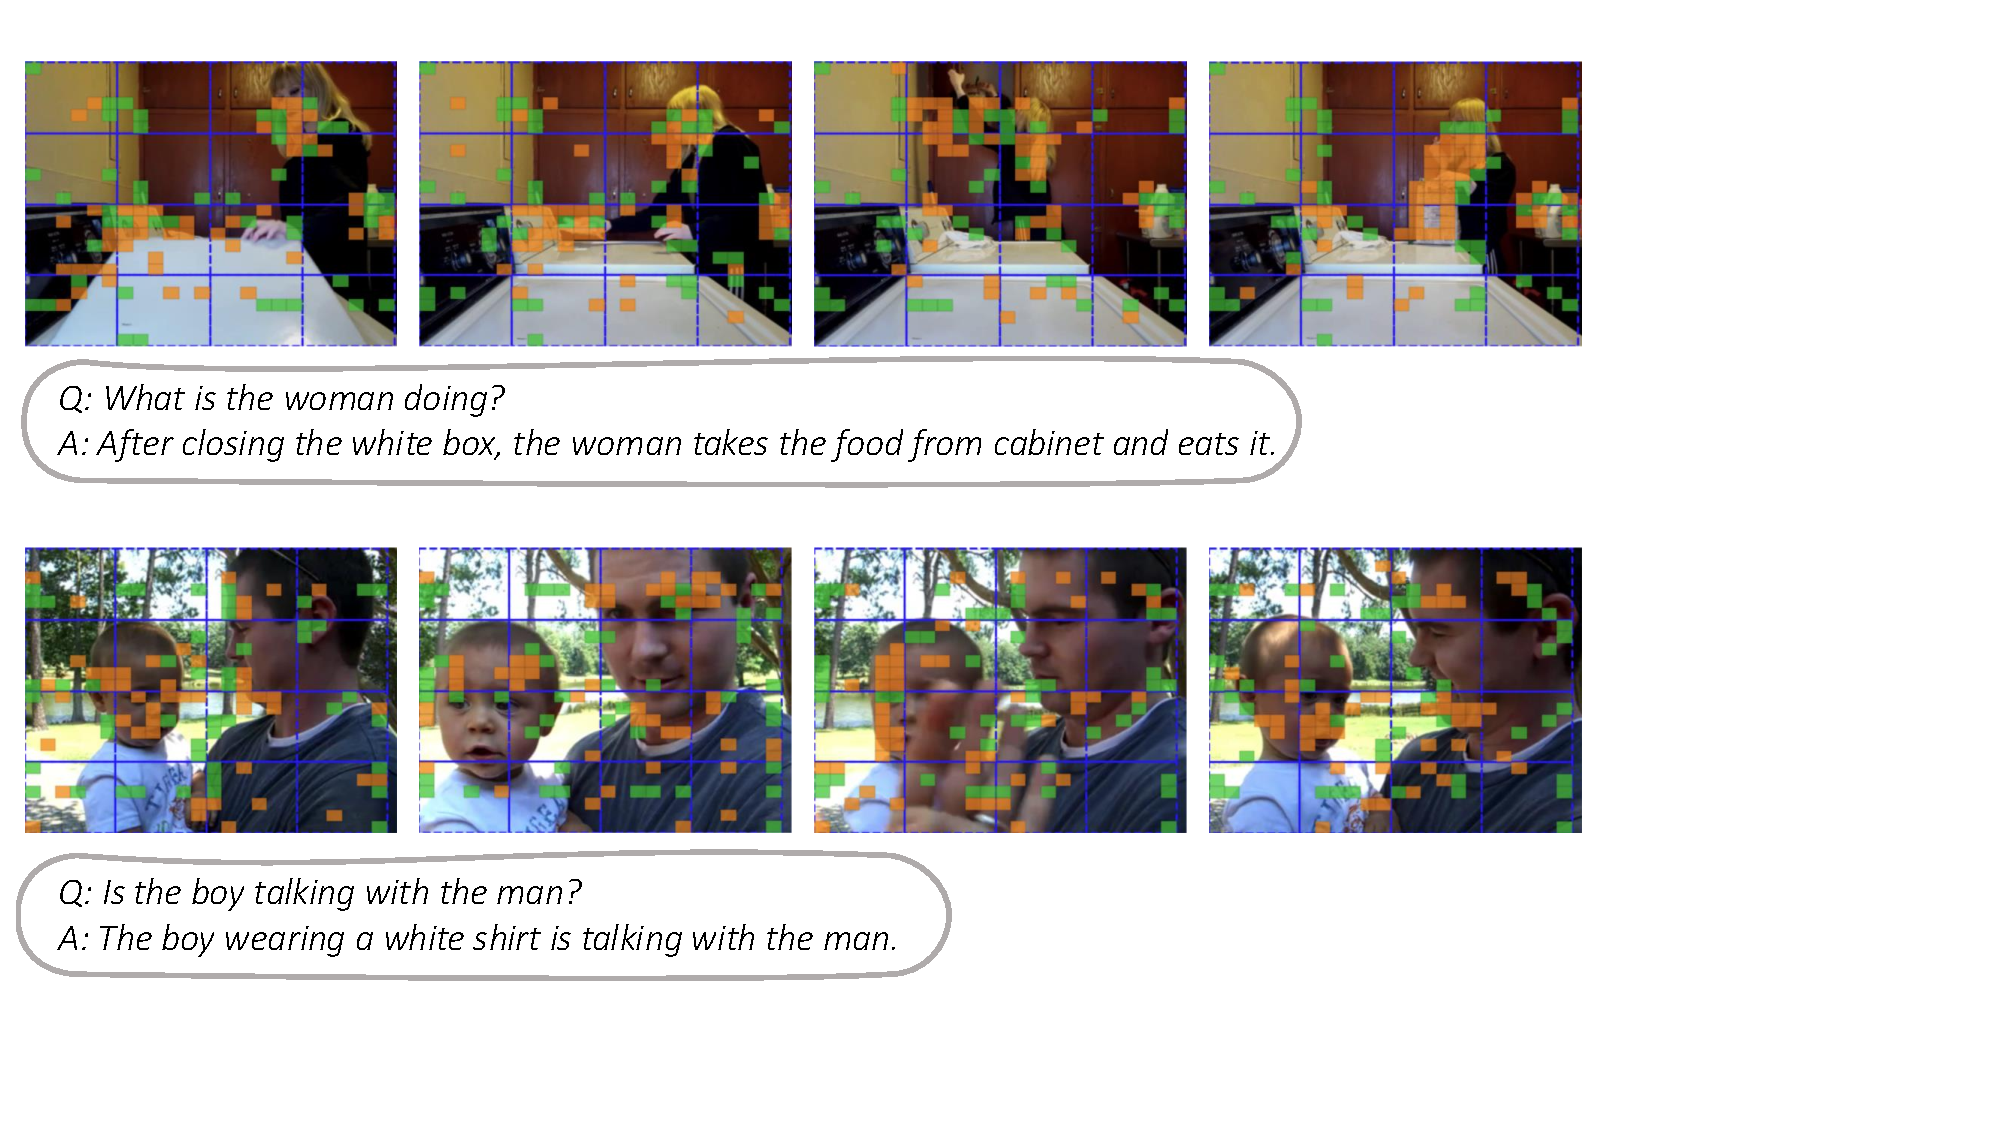
\includegraphics[width=\linewidth]{figs/cvpr2026_vis_fig.pdf}
    \vspace{-0.4cm}
    % \vspace{-0.4cm}
    \caption{Qualitative visualizations of our \textcolor{green}{Local}-\textcolor{orange}{Global} token anchors evolution across consecutive frames while optimal transport is adopted to aggregate necessary information from unselected tokens to help LLM precess better.}
    \label{fig:vis_cases}
    \vspace{-0.4cm}
\end{figure}

